\documentclass{article}
\usepackage[utf8]{inputenc}
\usepackage[cm]{fullpage}
\usepackage[]{graphicx}
\usepackage{indentfirst}
\usepackage{nopageno}


% Style choices, indent and text spacing
\setlength{\parindent}{8ex}
\renewcommand{\baselinestretch}{1.14}


\title{\textbf{CS-483: Wikipedia Scraping}}
\author{Grant Wade (grant.wade@wsu.edu)}
\date{August 15th, 2017}

\begin{document}
\maketitle

\section*{Overview:}
The goal of this project was to use the Wikipedia API to request data on
a topic that we want to learn about The topic that I decided to work with
was \textit{Linux software}. I think this could be an interesting topic to
work with because there is such a multitude of tools that can be used in a
Linux system; it can be hard to find the exact one you are looking for.
I'm hoping with this database it will be possible to create an easy way to
lookup different sub-categories of \textit{Linux software} to potentialy 
find software that will be useful, or interesting to work with. It is a very
broad category that has a total of 6846 pages and 1833 images at the time
of retreval. A portion of these pages don't have data that applies to the
topic because of how broad a lot of the Wikipedia categories can be.

\section*{How it's done:}
To start off with the script needs a category to begin its searching at.
Then it recursivly collects all titles of pages in the category and each
sub-category until it has collected every title. There checks in place to
make sure it doesn't end up in a endless loop of categories. After retrieval
of titles duplicates are removed, and the data collection begins. First, a
summary of the page is retrived, then all the categories that page is in,
then an image URL if one exists on the page, then the page view count, 
and lastly the images are downloaded into a directory for later use. 
Once all the data is collected an SQLite database is created and all the
data is placed into a table with the title of the page being the key,
since each Wikipedia page title is unique.

\section*{Example:}
This is the small example that is built into the wikipedia-scraping.py
script that will collect all the pages in the category Office suites for Linux
and then retrives the summary, categories, and a picture if one is found
then puts all that data in the database wiki-scraping.db under the table
Office suites for Linux.

\begin{center}
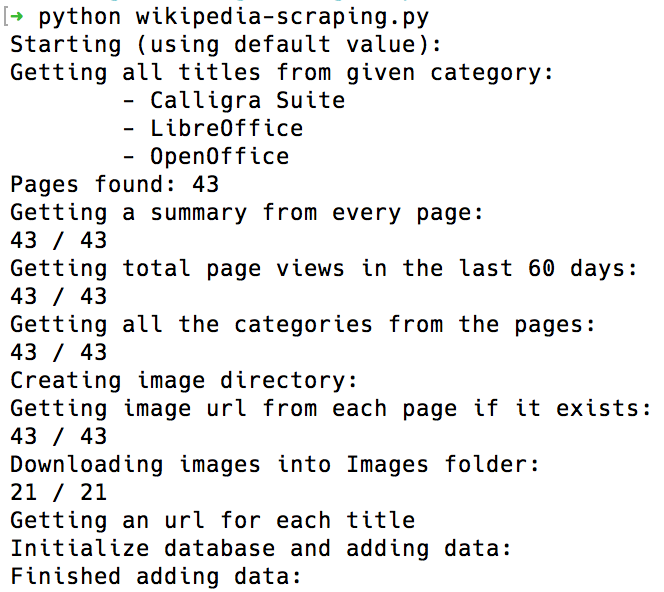
\includegraphics[width=.4\textwidth]{example.png}
\end{center}

\end{document}

